\chapter{Requirements}
\label{chap:requirements}

This chapter introduces the pulverization approach by explaining the terminologies and concepts that will be used in the rest of the thesis.
The logic that governs pulverization will be discussed by going on to give some examples of pulverized systems.
Next, the requirements that the framework must have to implement and concretize the pulverization concepts are reported. Finally, the
chapter concludes by reporting some relevant scenarios in which it makes sense to test the effectiveness of the framework.

\section{Pulverization domain model}
\label{sec:pulverization-domain-model}

Pulverization is an approach to conceive self-organization in distributed systems that facilitate deployment independence, i.e., the ability of an
application to run with no change on various deployments while retaining its original functional semantics.
The main idea is to organize the structure and the behaviour of a system in a way that the developer can focus on the logical model, abstracting from
the deployment details, scheduling and communication.
The logical model can be partitioned into a set of software components that can be deployed on the available infrastructure, while the application
logic will preserve the functional goals independently from the actual deployment.

To better formalize the terminology coming from the pulverization, the following ubiquitous language is proposed in~\Cref{tab:ubiquitous-language}.

\begin{table}
	\begin{tabularx}{\textwidth}{l X}
		\toprule
		\textbf{Concept}          & \textbf{Definition}                                                                                             \\
		\midrule
		Sensors                   & Component that represents a set of logical \emph{sensors}                                                       \\
		Actuators                 & Component that represents a set of logical \emph{actuators}                                                     \\
		Behaviour                 & Component that models the device behaviour                                                                      \\
		Communication             & Component that handles the interaction with neighbours (other devices)                                          \\
		State                     & Component the holds the representation of the device's knowledge                                                \\
		Thin host                 & A device that has limited computational power and memory                                                        \\
		Thick host                & A device that has a powerful computational power and memory                                                     \\
		Logical device            & A logical representation of a device composed of several components which they can be deployed on the available
		infrastructure                                                                                                                              \\
		Logical neighbouring link & Defines a logical connection between two logical devices defining the network topology.
		The aforementioned structure can change over time.                                                                                          \\
		\bottomrule
	\end{tabularx}
	\label{tab:ubiquitous-language}
	\caption{Pulverization Ubiquitous language.}
\end{table}

\begin{figure}
	\centering
	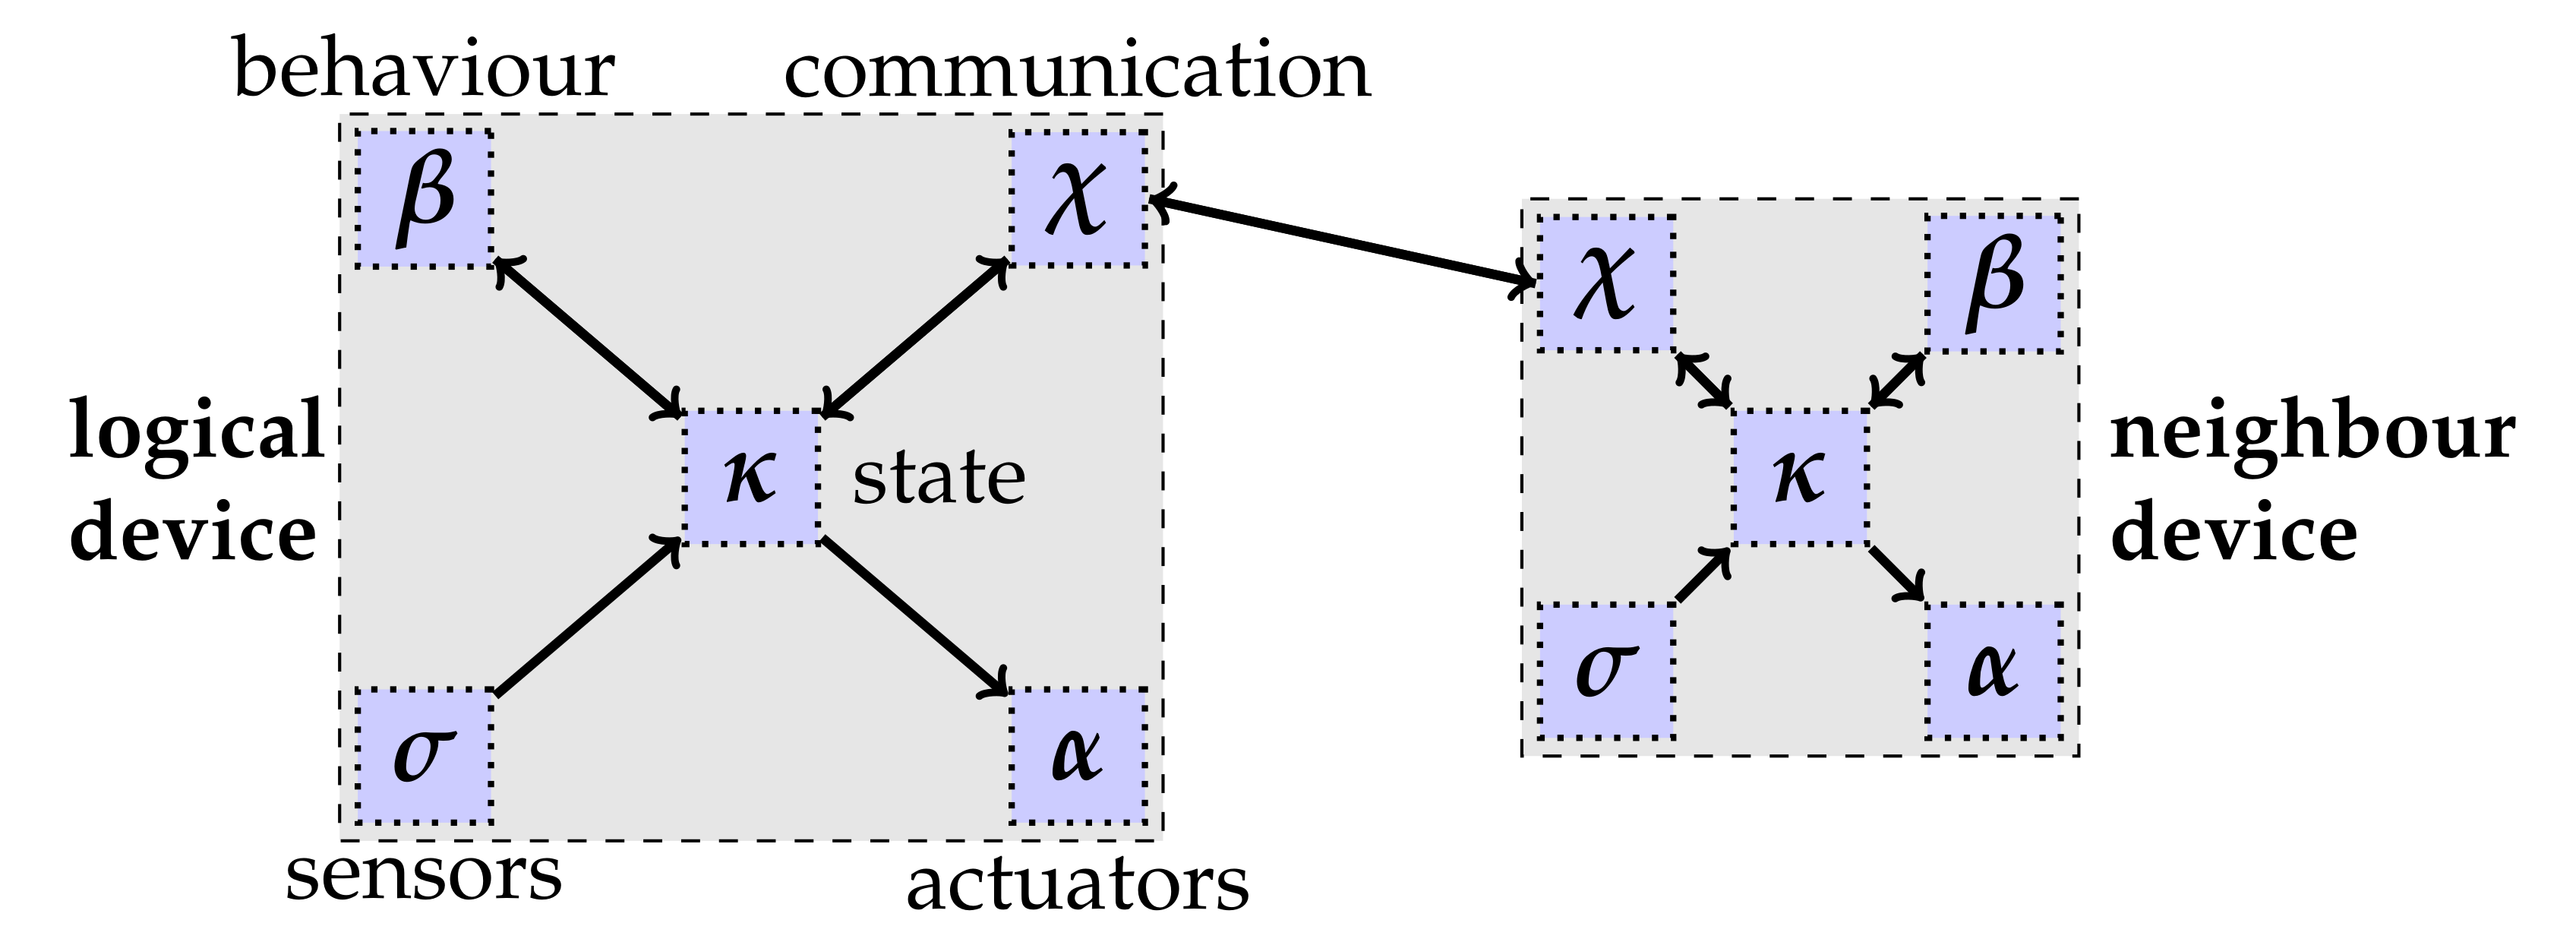
\includegraphics[width=\textwidth]{figures/original-components-interactions.png}
	\caption{Representation of a logical device split into its components and a connection with one of its neighbours}
	\label{fig:logical-device}
\end{figure}

Henceforth, concepts characterizing pulverization will be used with the meaning given in~\Cref{tab:ubiquitous-language}.

A \emph{Logical Device} is the representation of a device in the system abstracting from the specific deployment details.
It is composed of \emph{five} components: \emph{Sensors}, \emph{Actuators}, \emph{Behaviour}, \emph{Communication} and \emph{State} while the
interaction between them determines the device's logic in the system. The~\Cref{fig:logical-device} shows a representation of a logical device
split into its components defining also a link with another device.

The \emph{Sensors} $\sigma$ and \emph{Actuators} $\alpha$ components represent the way the device interacts with the environment: the former is used
to acquire information from the environment, while the latter is used to actuate on the environment.
The \emph{State} $\kappa$ component represents the device's knowledge and abstract from the actual storage mechanism or representation.
The \emph{Communication} $\chi$ component handles the interaction with neighbours by holding the information about the identity of the neighbours and
how to reach them. The send and receive operations occur through respectively the \emph{input channels} and the \emph{output channels}, where the
output channel of a device is connected to the input channel of its neighbours.
Finally, the \emph{Behaviour} $\beta$ component models the device behaviour via a \emph{function} which maps the state of the device to a new state,
defines a set of prescriptive actions to be performed and a set of coordination data to be propagated to the neighbours.

Each device performs a MAPE-like cycle that includes the following steps and that defines the interactions between the device's subcomponents as
depicted in~\Cref{fig:logical-device}, where the arrows denote the message flow:

\begin{enumerate}
	\item \textbf{Context acquisition:} the device acquires information from its sensors and communications, storing them in the device state
	\item \textbf{Computation:} the device behaviour function is computed against the device state
	\item \textbf{Coordination data propagation:} coordination data is set to all the device neighbours
	\item \textbf{Actuation:} the actuators are activated to execute a set of prescriptive actions
\end{enumerate}

A platform is a collection of physical \emph{hosts} connected by a dynamic graph of physical network links, representing the communication channel
between two hosts. A host is an entity with a unique identifier (e.g. an IP address, URI resource, etc.) and can be a computer system, an embedded
device holding sensors and actuators, a virtual machine or a software container. The type of communication channel (the link between hosts) may
vary depending on the underlying network infrastructure and protocols.
The \emph{hosts} types are divided into two categories: \emph{thin hosts} and \emph{thick hosts}. Thin hosts are devices with limited computational
power and memory, while thick hosts can compute and may even do so on behalf of multiple logical devices.

\begin{figure}
	\centering
	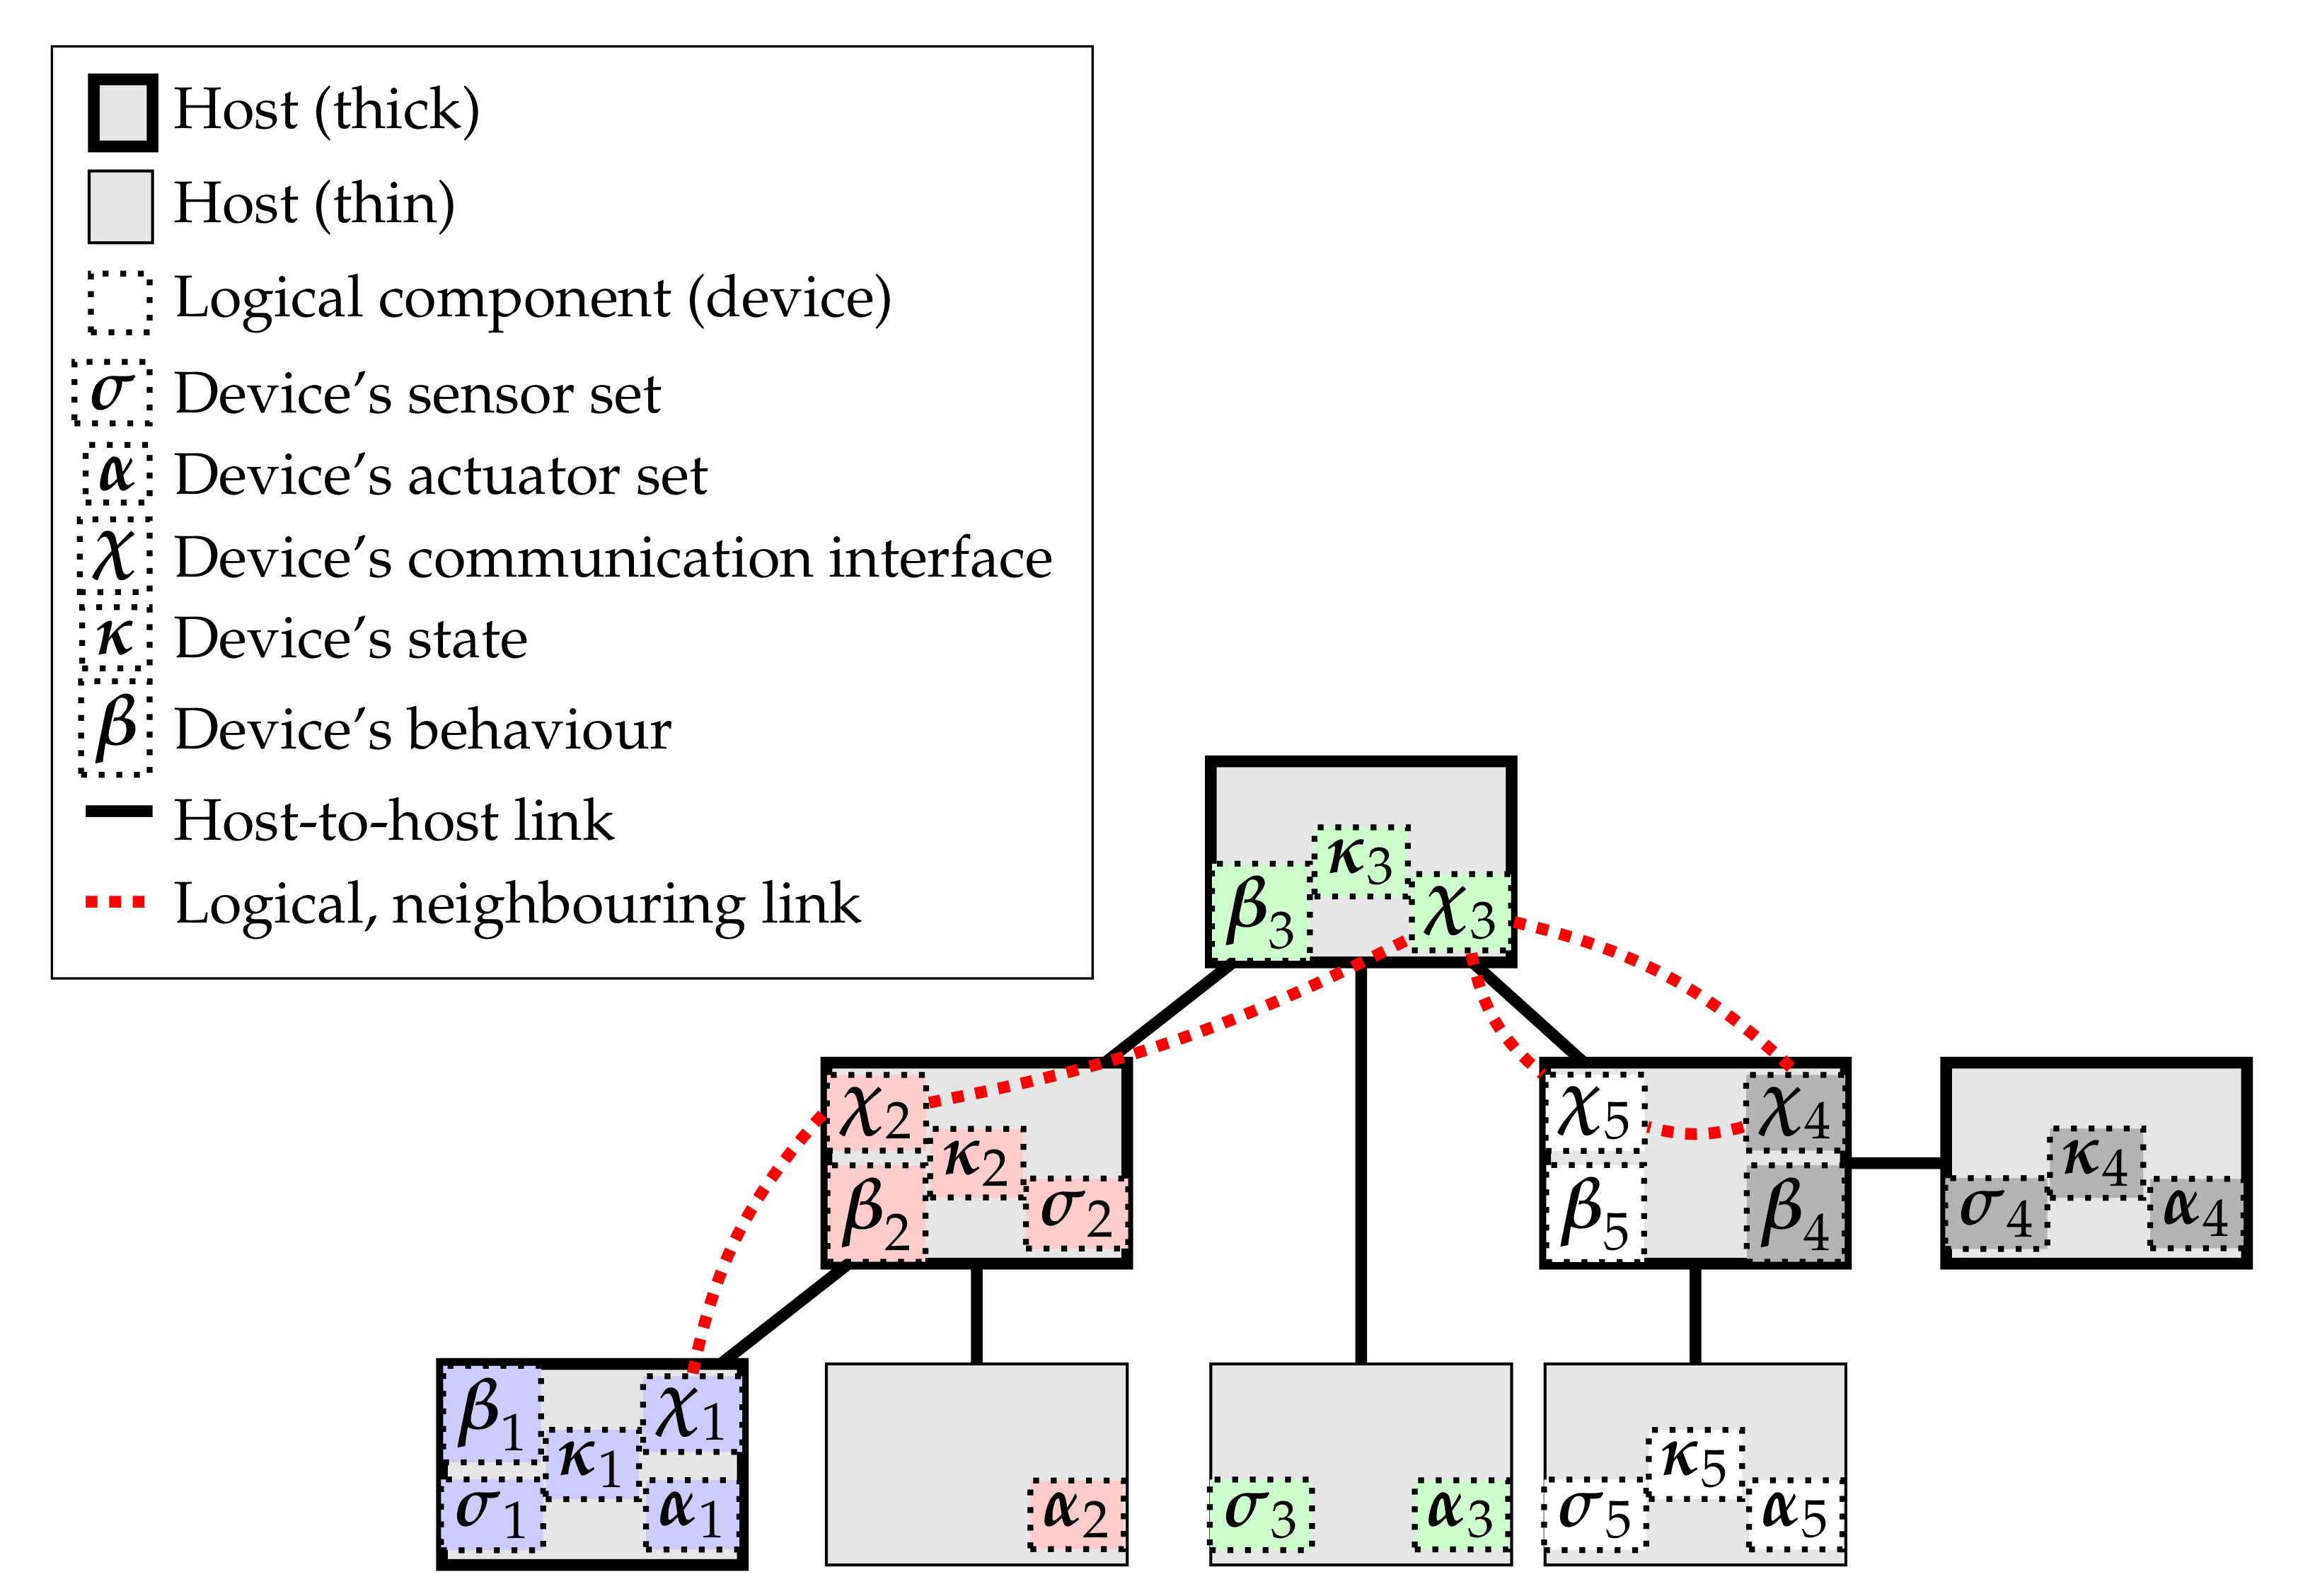
\includegraphics[width=0.7\linewidth]{figures/cps-example.png}
	\caption{Example of instantiation of the CPS model.}
	\label{fig:cps-example}
\end{figure}

\begin{figure}
	\centering
	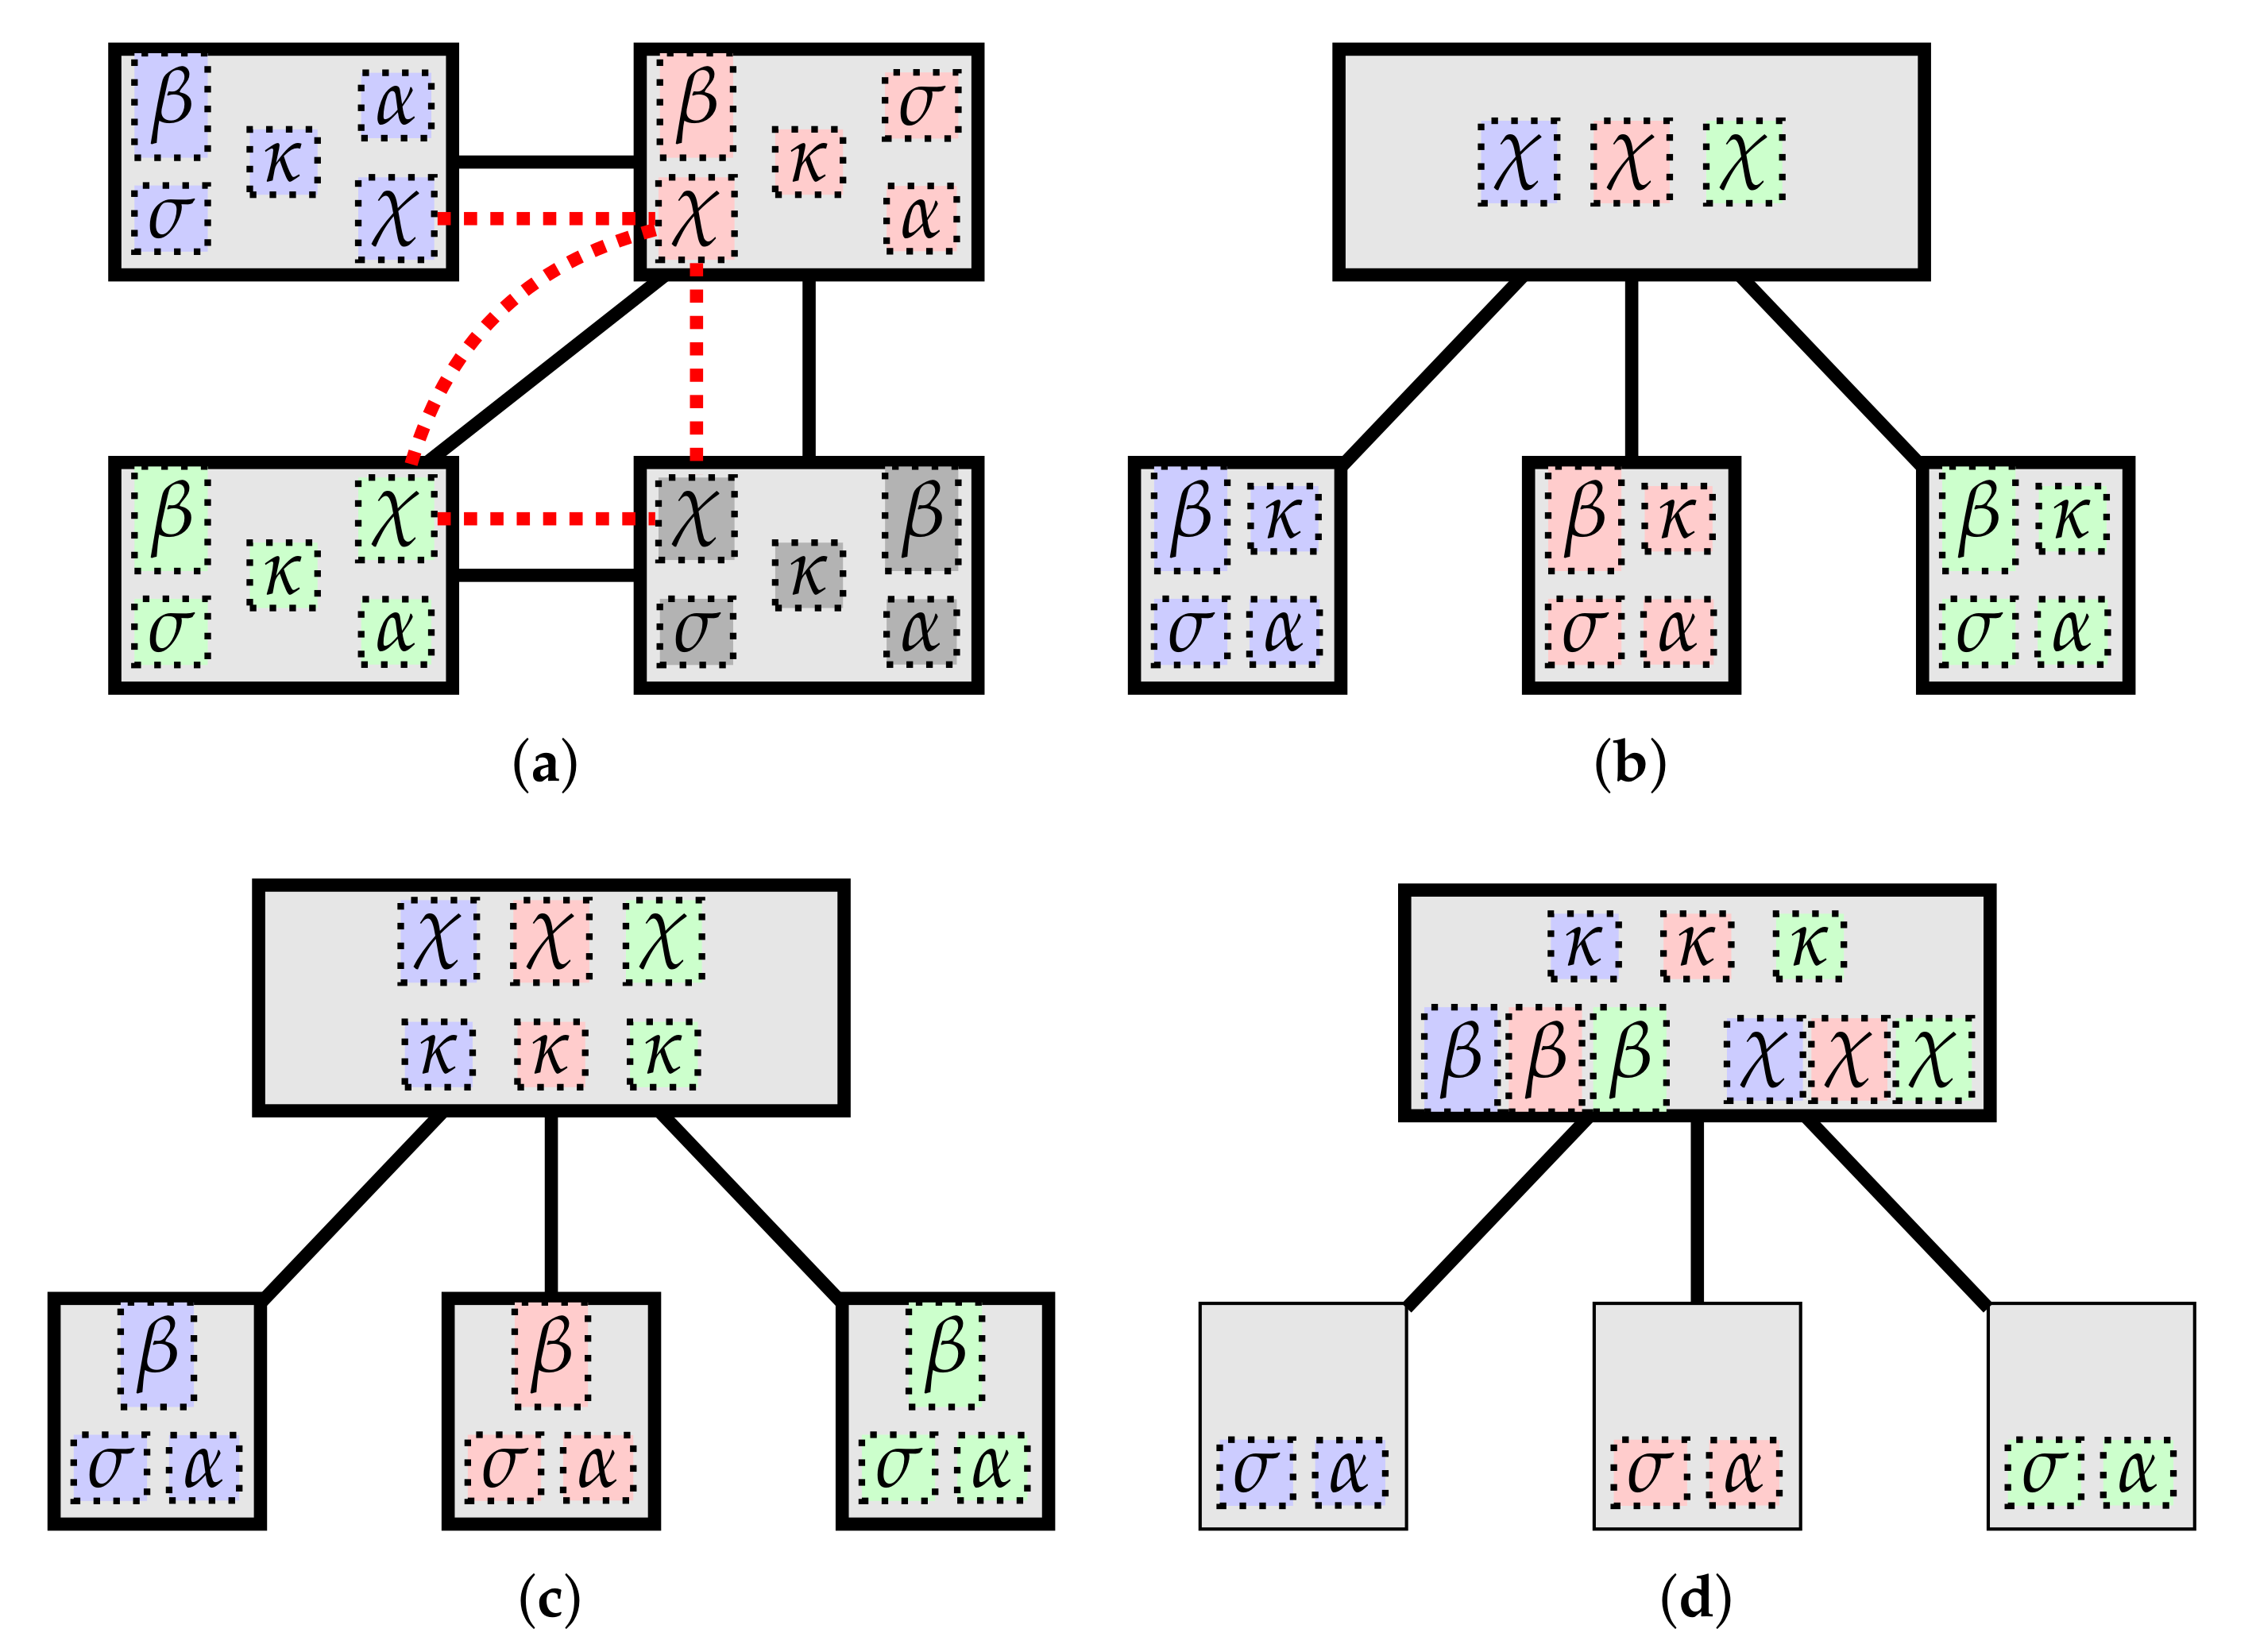
\includegraphics[width=0.7\linewidth]{figures/notable-deployments.png}
	\caption{\textbf{(a)} Peer-to-peer style; \textbf{(b)} broker-based style (e.g. MQTT); \textbf{(c)} Big data in the cloud style; \textbf{(d)} embedded device with sensors/actuators.}
	\label{fig:notable-deployments}
\end{figure}

The deployment of the CPS can be defined as an \emph{allocation map} placing each component of each device to specific hosts in the platform.
An example of a deployment can be seen in~\Cref{fig:cps-example}. In the example is assumed that all the sensors and actuators are deployed on the
same host, though this is not a requirement, sensors and actuators may be deployed on different hosts.

Examples of deployment are provided in~\Cref{fig:notable-deployments} showing an increasing number of responsibilities are centralized.
The~\Cref{fig:notable-deployments}a shows a peer-to-peer style deployment where, for each device, all the components are deployed on the same host.
This style is not suitable in a sensor network where a device is designed to operate for a long time using solely battery power and is not equipped
with enough power to host a $\beta$-component.
The~\Cref{fig:notable-deployments}b shows a broker-based style deployment where all the $\chi$-components are deployed on a separate host (broker).
This is a common scenario in IoT systems where a broker is used to handle the communication between devices.
The~\Cref{fig:notable-deployments}c shows big data in the cloud style deployment where all the $\kappa$-components are deployed in the cloud
enabling big-data analysis.
The~\Cref{fig:notable-deployments}d shows an embedded device with sensors/actuators style deployment where all the $\alpha$ and $\sigma$-components
are deployed on the same thin host while all the remaining components are deployed on a thick host. This scenario covers the case of a device
with limited computational power and memory by offloading the $\beta$-component to a thick host.

% - New section ---------------------------------------------------------------

\section{Framework requirements}
\label{sec:framework-requirements}

% - New section ---------------------------------------------------------------

\section{Reference scenarios}
\label{sec:reference-scenarios}
